\section{Context}

\subsection{NTT DATA}

\textbf{NTT DATA} has a rich history spanning over 50 years, rooted in the establishment of Japan's first telegraph service. The company's evolution into a major player in the IT industry began in 1967 with the formation of its Data Communications Division. Subsequent milestones include privatization in 1985 and the spin-off from NTT in 1988, leading to its emergence as a leading information and communication service company in Japan.\\

In 1992, NTT data procured 6 million smart cards at a time where the annual shipment was still only in the hundreds of thousands. One year later, the company received the \textbf{Deming Application Prize} 1993, which  is the longest-running and one of the highest awards in the world,  and is a first for the information service industry.\\

From 2005 to 2016, NTT DATA embarked on a Global Strategy Period, aiming to establish itself as a "Global IT Innovator." This phase saw the company expanding its presence internationally, forming strategic alliances, and engaging in mergers and acquisitions to strengthen its global footprint.\\

In the current Global 3rd Stage, which began in 2017, NTT DATA is focused on becoming a "Trusted Global Innovator." This involves accelerating digital initiatives, enhancing profitability outside Japan, and fostering innovation through partnerships and cutting-edge technologies. \\

Through its long history of innovation, strategic expansion, and a commitment to excellence, NTT DATA continues to lead the way in shaping the future of the IT industry on a global scale.\\

\newpage
\subsection{Company presentation}

NTT DATA is a global company providing IT services and consulting, part of the NTT Group (Nippon Telegraph and Telephone Corporation), one of the largest telecommunications conglomerates in the world. Founded in Japan in 1967, NTT DATA offers a comprehensive range of IT services and technological solutions to clients worldwide.\\

As an IT service provider, NTT DATA offers strategy consulting services, application development services, system integration services, IT infrastructure services, business process management (BPM) services, business process outsourcing (BPO) services, and technology infrastructure management services. They work with companies from various sectors, including finance, healthcare, telecommunications, utilities, automotive, and many others.\\

NTT DATA is recognized for its technical expertise, innovation capabilities, and commitment to providing customized solutions that meet the specific needs of its clients. The company leverages emerging technologies such as artificial intelligence, data analytics, the Internet of Things (IoT), and cloud computing to help its clients improve operational efficiency, innovate, and remain competitive in the market.

\begin{figure}[h!]
	\centering
	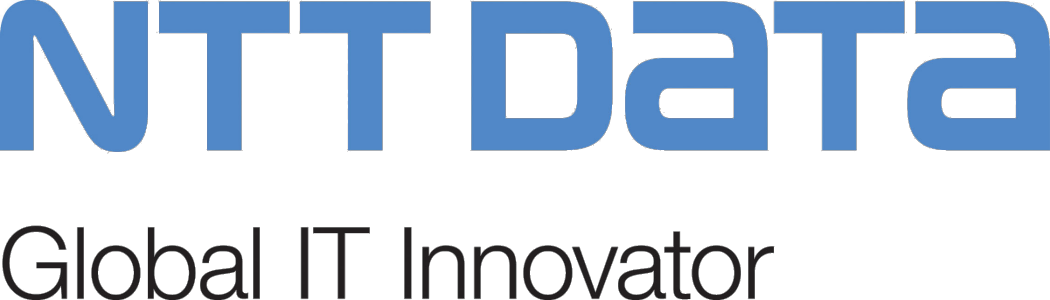
\includegraphics[width=0.8\linewidth]{Image/nttgloballogo.png}
	\caption{NTT DATA Logo}
	\label{fig:NTT DATA Logo}
\end{figure}
\pagebreak

\subsection{Company historic}

Before delving into the detailed history of NTT DATA, it is worth noting that the company has experienced significant growth and evolution since its establishment in 1967. From its humble beginnings as a subsidiary of NTT, NTT DATA has grown into a leading global company in the IT services and consulting sector. Here is a summary of the key milestones in its historical journey:

\begin{figure}[h!]
	\centering
	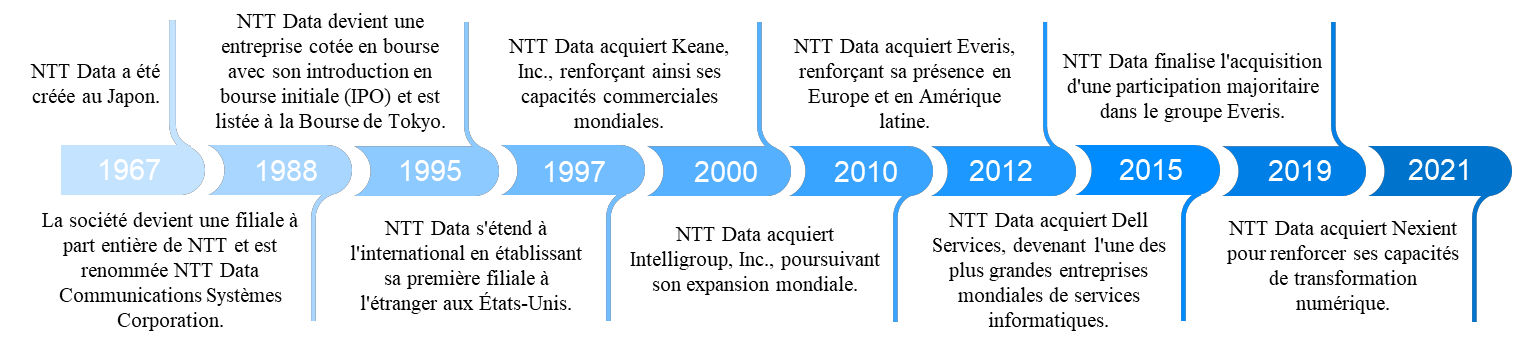
\includegraphics[width=0.8\linewidth]{Image/ntthistoric.png}
	\caption{NTT DATA historic}
	\label{fig:NTT DATA historic}
\end{figure}

Today, NTT DATA is recognized as one of the global leaders in IT services and consulting, providing innovative technological solutions to its clients worldwide.

\subsection{Global presence}
NTT DATA has a broad global presence with offices and service delivery centers in many countries around the world.
\begin{figure}[h!]
	\centering
	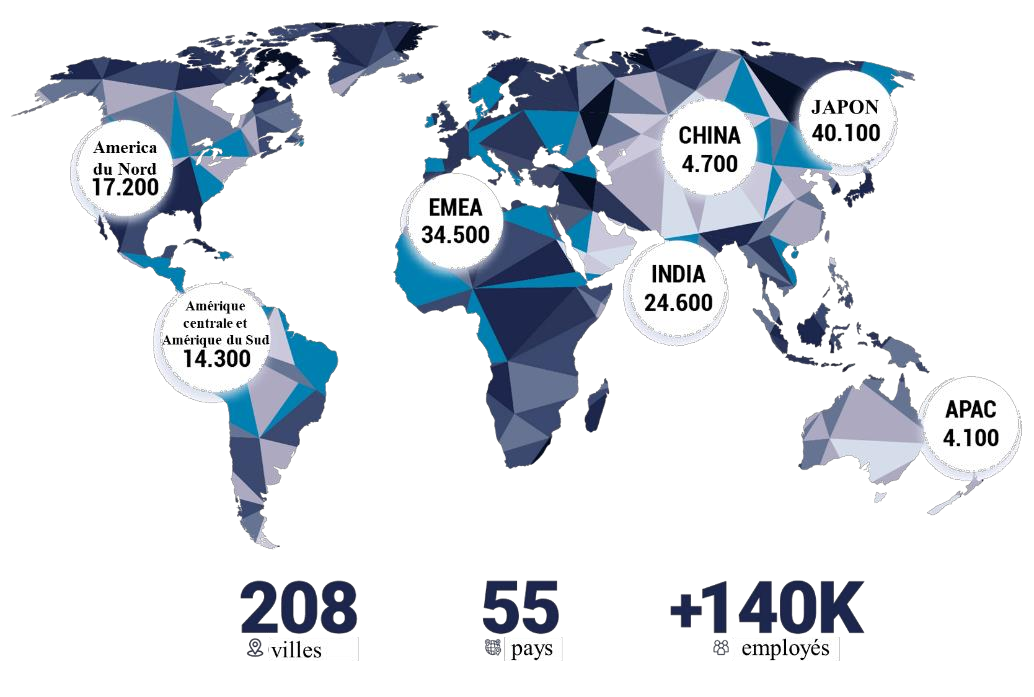
\includegraphics[width=0.8\linewidth]{Image/nttmap.png}
	\caption{NTT DATA historic}
	\label{fig:NTT DATA historic}
\end{figure}

\pagebreak
\subsection{Company sector activities}

NTT DATA collaborates with various industries, providing tailored IT solutions and consulting services to address specific challenges and enhance operational efficiency. Here are some key sectors in which NTT DATA is actively involved:

\begin{itemize}
	\item Financial Services: NTT DATA works with financial institutions, banks, insurance companies, and other financial sector players to deliver IT solutions and consulting services aimed at improving operational efficiency, risk management, customer experience, and regulatory compliance.
	 
	\item Healthcare and Life Sciences: NTT DATA offers technological solutions to healthcare providers, pharmaceutical companies, and medical research organizations. This includes electronic medical record management, healthcare management systems, health data analytics, telemedicine services, and clinical trial monitoring solutions.
	
	\item Public Sector: NTT DATA collaborates closely with governments and public sector organizations to provide IT solutions and consulting services that enhance public service delivery, data management, public safety, resource management, and administrative efficiency.
	
	\item Manufacturing and Automotive: NTT DATA provides technological solutions to manufacturers and automotive companies to optimize manufacturing operations, improve supply chain management, integrate the Internet of Things (IoT) into production processes, and develop smart mobility solutions.
	
	\item Telecommunications and Media: NTT DATA partners with telecommunications service providers and media companies to deliver IT infrastructure solutions, digital transformation services, data analytics solutions, online service platforms, and customer management solutions.
	
	\item In addition to these specific sectors, NTT DATA also works with businesses across various industries such as energy, transportation, retail, travel, and hospitality, providing customized IT services and solutions tailored to their specific needs.
\end{itemize}

\begin{figure}[h!]
	\centering
	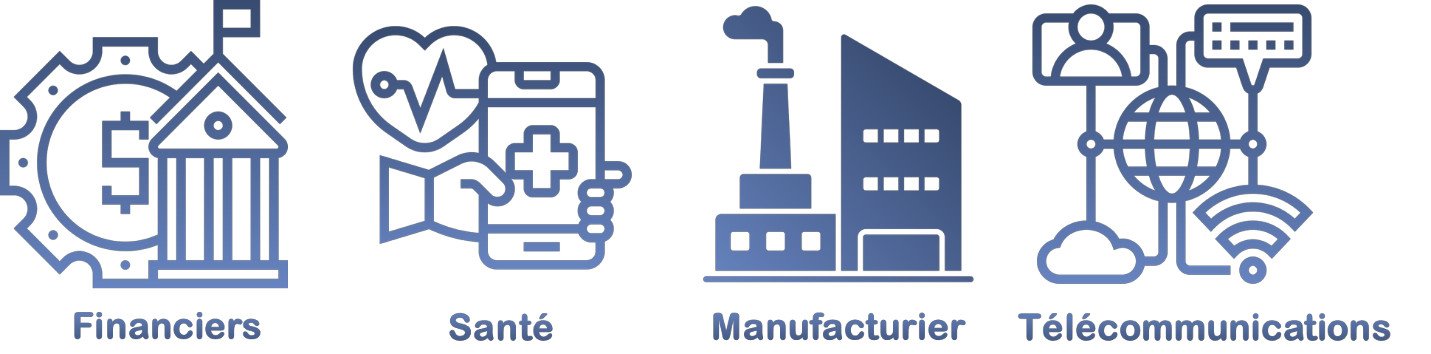
\includegraphics[width=0.8\linewidth]{Image/nttsector.png}
	\caption{NTT DATA sectors}
	\label{fig:NTT DATA sectors}
\end{figure}

\pagebreak

\subsection{Company services}

NTT DATA, as a trusted global provider of IT services, offers a comprehensive range of services to assist businesses in tackling digital challenges and fostering innovation. The following figure illustrates the services provided by NTT DATA:
\begin{figure}[h!]
	\centering
	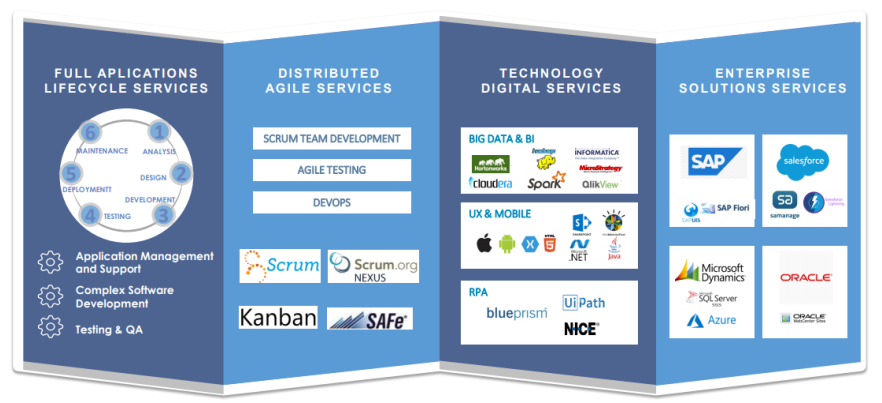
\includegraphics[width=0.8\linewidth]{Image/nttactivities.png}
	\caption{NTT DATA activities}
	\label{fig:NTT DATA activities}
\end{figure}

\subsection{Partners}


NTT DATA has established strategic partnerships with numerous leading technology and service companies. These partnerships are essential for enhancing NTT DATA's solution offerings and providing added value to its clients. Key partners include industry giants such as Microsoft, Oracle, SAP, Salesforce, IBM, and Amazon Web Services (AWS). These partnerships enable NTT DATA to access the latest technologies and deliver innovative solutions in areas such as cloud computing, enterprise software, customer relationship management, data analytics, and more. Through these strategic partnerships, NTT DATA can offer consulting, integration, and solution management services based on the platforms and technologies of its partners, thereby meeting the diverse needs of its clients across various industries.



\begin{figure}[h!]
	\centering
	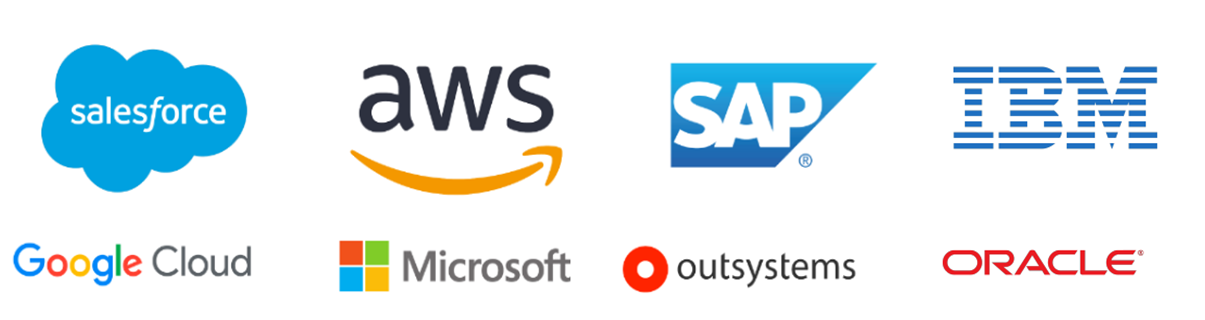
\includegraphics[width=0.8\linewidth]{Image/nttpartners.png}
	\caption{NTT DATA partners}
	\label{fig:NTT DATA partners}
\end{figure}

\pagebreak
\subsection{Clients}

NTT DATA's clients encompass a wide range of businesses and organizations worldwide. Leveraging its technological expertise and innovative solutions, NTT DATA has forged lasting partnerships with clients across various sectors including finance, telecommunications, healthcare, manufacturing, and more. Whether serving multinational corporations or local enterprises, NTT DATA is committed to delivering high-quality services tailored to the specific needs of each client. The primary goal is to establish long-term trust-based relationships and contribute to the success and growth of its clients. Here are some of NTT DATA's key clients:


\begin{figure}[h!]
	\centering
	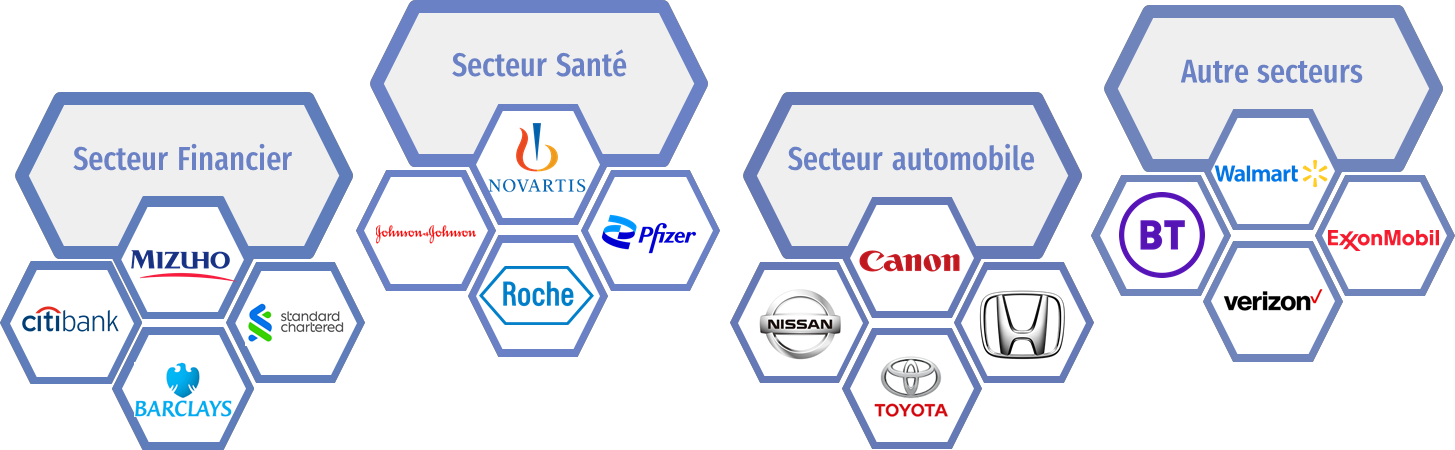
\includegraphics[width=0.8\linewidth]{Image/nttclients.png}
	\caption{NTT DATA clients}
	\label{fig:NTT DATA clients}
\end{figure}


\subsection{Technologies}


NTT DATA employs a wide array of technologies to execute and evolve application services for its clients. Among the key technologies utilized are Java, .NET, SQL, Cobol, testing (software testing), and Robotic Process Automation (RPA). These technologies are implemented by a highly skilled and talented team specialized not only in technical aspects but also in industry knowledge. By combining these cutting-edge technologies with deep industry expertise, NTT DATA is able to deliver innovative solutions tailored to the specific needs of its clients, while ensuring high quality and optimal productivity in the execution of their application projects.

\begin{figure}[h!]
	\centering
	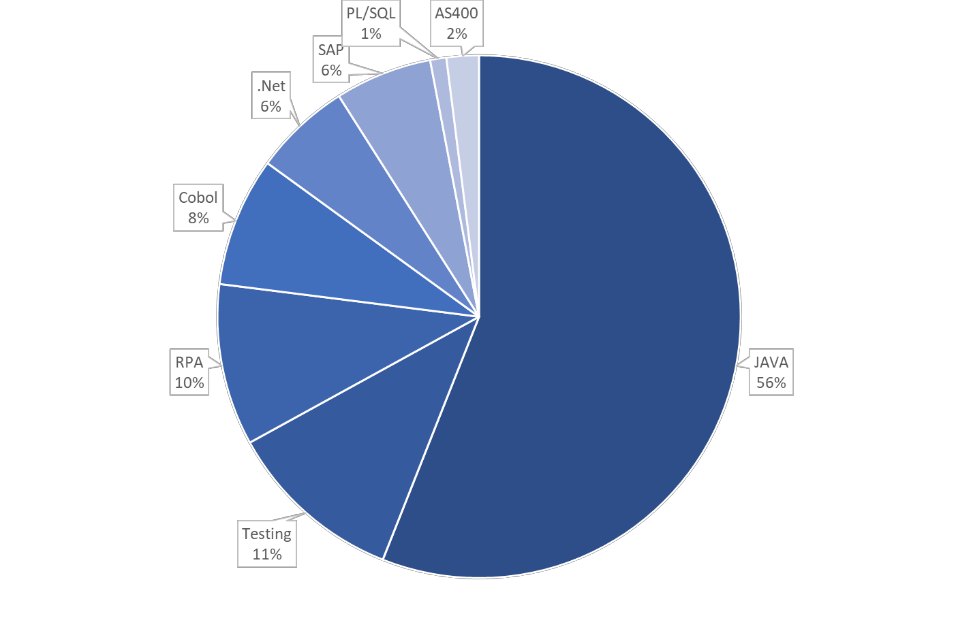
\includegraphics[width=0.65\linewidth]{Image/ntttechnologies.png}
	\caption{NTT DATA technologies}
	\label{fig:NTT DATA technologies}
\end{figure}

\pagebreak


\subsection{NTT DATA in Morocco}

NTT DATA Morocco is a subsidiary of NTT DATA Corporation, a global provider of IT services and technological solutions. The company offers a comprehensive range of services, including software development, IT infrastructure management, technology consulting, digital transformation, and more.\\

NTT DATA Morocco collaborates with local and international clients across various industries such as finance, telecommunications, healthcare, manufacturing, public sector, retail, and other industries. The goal of NTT DATA Morocco is to help businesses optimize their operations, improve efficiency, and address the technological challenges they face.\\

As a subsidiary of NTT DATA Corporation, NTT DATA Morocco benefits from the company's global expertise and experience in the field of information technology. This enables it to offer cutting-edge solutions and innovate in the field of IT services to meet the specific needs of the Moroccan market.\\

NTT DATA Morocco also contributes to the country's technology ecosystem by collaborating with local partners, universities, and institutions to promote innovation, skill development, and growth in the information technology sector in Morocco.


\subsection{Organizational chart}

***

\subsection{Career model}


NTT DATA employs a career model to enable employees to develop their skills, progress professionally, and achieve their career goals within the company.

The NTT DATA career model is characterized by the following aspects:

\begin{figure}[h!]
	\centering
	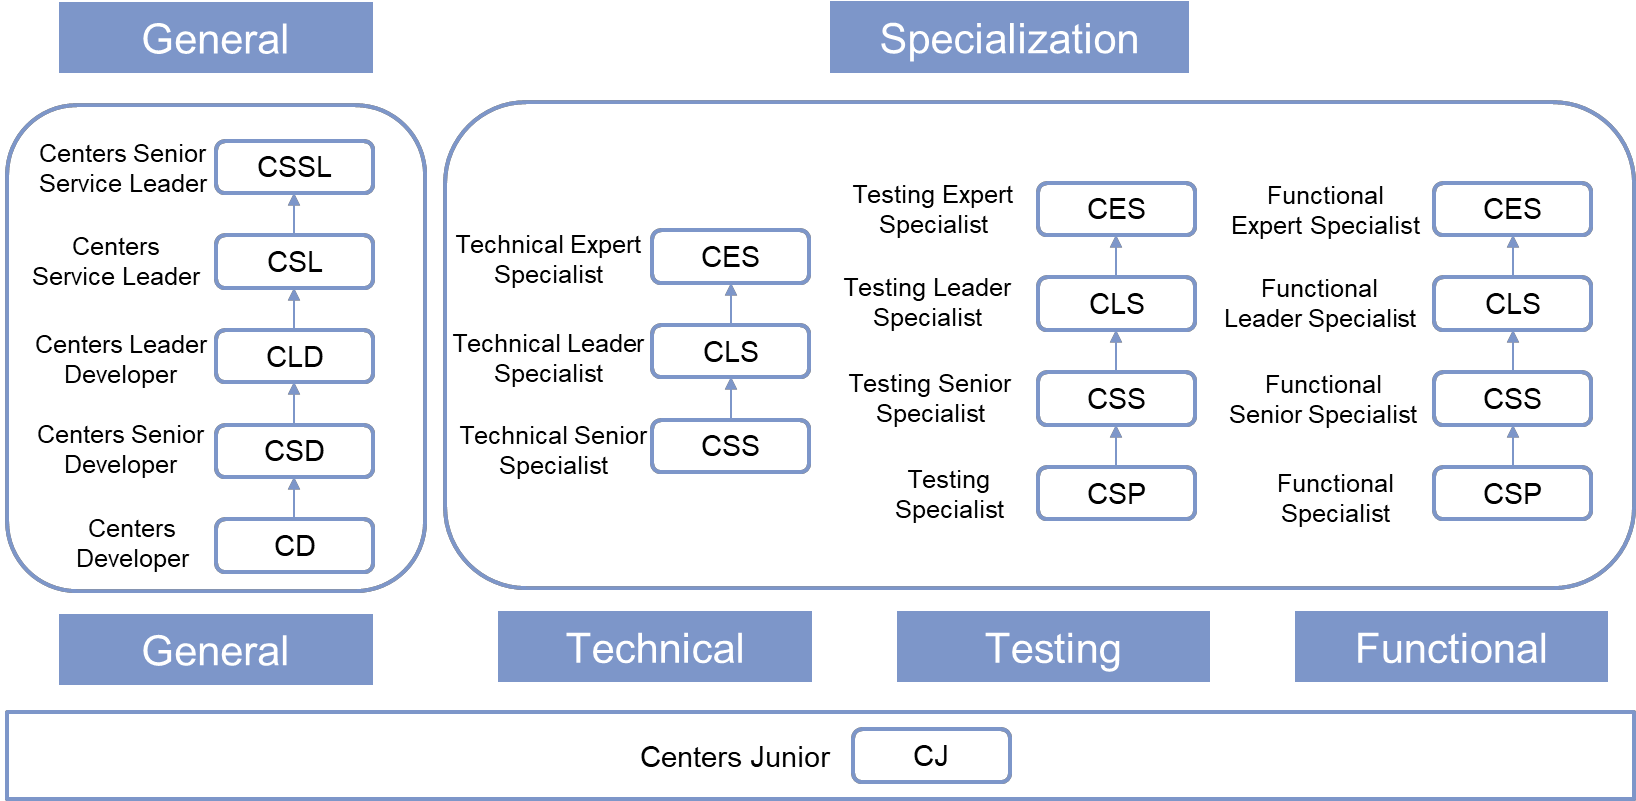
\includegraphics[width=0.65\linewidth]{Image/nttcareer.png}
	\caption{NTT DATA careers}
	\label{fig:NTT DATA careers}
\end{figure}


\subsection{Societal and environmental responsability}


Talk about environnement with cloud minimal use, the gain when mooving to pgsql ? The less use of processing/computing.

gender equality (including IT)


multi-cultural space +ieurs languages (spanish + arabic + english here)

\subsection{Problematic}


The human ressources and staffing workers were using non efficient nor pratictical way to manage employees and clients of the company.\\
Using Excel files to store a huge amount of data with the possibility of error and not necesseraly normalized pratice, this method wasn't maintainable nor evolutive.\\

A fragment of an application had been realized, using \textbf{Elasticsearch} as \textbf{database} to manage all the data contained in multiple Excel files. However maintaining Elasticsearch clusters requires expertise and careful planning to ensure optimal performance and reliability. Additionally, while Elasticsearch offers powerful search and analytics capabilities, it may not be as feature-rich in certain areas compared to traditional relational databases, such as complex transactional support. Finally, Elasticsearch's distributed nature can introduce challenges in terms of data consistency and coordination, particularly in scenarios with high write throughput or when dealing with network partitions without forgetting the higher amount of processing required.\\

The company wants a web application that can help its workers and to manage each one of the processes.
